% Matematica das Coisas
% Exemplo LaTeX
% 2021/2022
% Ana Jacinta Soares
%%%%%%%%%%%%%%%%%%%%%%%%%%%%%%%%

\documentclass[11pt,a4paper]{article}
\usepackage[dvipdf]{epsfig}
\usepackage{amsfonts,amsmath,amssymb,amsthm}
\usepackage[portuges]{babel}
\usepackage{color}
\usepackage{enumerate}
\usepackage{hyperref}
%\usepackage[applemac]{inputenc}   % para acentos no Mac
\usepackage[T1]{fontenc}              % para acentos noutros computadores
% \usepackage[utf8]{inputenc}          % para acentos noutros computadores
\usepackage[gen]{eurosym}
\usepackage{enumerate}

%%%%%%%%%%%%%
% Para definir a mancha de texto e a sua posicao
\hoffset -0.7in
\voffset -0.5in
\addtolength{\textwidth}{3.5cm}
\addtolength{\textheight}{2cm}

%%%%%%%%%%%%%%%%%%%
% Simbolos
\def\RR{\mathbb R}
\def\QQ{\mathbb Q}
\def\NN{\mathbb N}
\def\ZZ{\mathbb Z}
\def\PP{\mathbb P}
\def\CC{\mathbb C}

\def\u{\mbox{\boldmath$u$}}
\def\v{\mbox{\boldmath$v$}}
\def\q{\mbox{\boldmath$q$}}

%%%%%%%%%%%%%%%%%%%
% Para definir cores

\definecolor{cinz}{cmyk}{0,0,0,.5}
\definecolor{cinzz}{cmyk}{0,0,0,.75}
\definecolor{violeta}{cmyk}{0.3,1,0,0}
\definecolor{cast}{cmyk}{0,.4,1,.4}
\definecolor{ggreen}{cmyk}{1,     0,      1,      0}
\definecolor{ror}{cmyk}{0, 0.77, 0.87, 0}
\definecolor{amber(sae/ece)}{rgb}{1.0, 0.49, 0.0}
\definecolor{navyblue}{rgb}{0.2, 0.2, 0.6}
\definecolor{azul}{rgb}{0.2, 0.29996, 0.8 }
\definecolor{myred}{cmyk}{0.1, 1, 0.5, 0}

%%%%%%%%%%%%%%%%%%%
% Teoremas e outros ambiente

\theoremstyle{plain}
\newtheorem{thm}{Theorem}[section]
\newtheorem{lem}{Lemma}[section]
\newtheorem{prop}[thm]{Proposition}
\newtheorem*{cor}{Corollary}

\theoremstyle{definition}
\newtheorem{defn}{Definition}[section]
\newtheorem{conj}{Conjecture}[section]
\newtheorem{exmp}{Example}[section]

\theoremstyle{remark}
\newtheorem*{rem}{Remark}
\newtheorem*{note}{Note}

%%%%%%%%%%%%%%%%%%%

\newcommand{\dps}{\displaystyle}
\allowdisplaybreaks[1]

%%%%%%%%%%%%%%%%%%%
% Operadores

\DeclareMathOperator{\sen}{sen}
%\DeclareMathOperator{\cos}{cos}
\DeclareMathOperator{\tg}{tg}
\DeclareMathOperator{\cotg}{cotg}

\DeclareMathOperator{\asen}{arcsen}
\DeclareMathOperator{\arcos}{arccos}
\DeclareMathOperator{\arctg}{arctg}
\DeclareMathOperator{\arccotg}{arccotg}

\DeclareMathOperator{\sh}{sh}
\DeclareMathOperator{\ch}{ch}
\DeclareMathOperator{\tah}{th}
%\DeclareMathOperator{\coth}{coth}

\DeclareMathOperator{\agc}{argch}
\DeclareMathOperator{\ags}{argsh}
\DeclareMathOperator{\agt}{argth}
\DeclareMathOperator{\agct}{argcoth}




%%%%%%%%%%%%%%
\usepackage{graphicx}

% Define figures como o path para as imagens.
\graphicspath{ {imagens/} }



% Informações do PDF
%\usepackage[pdftex,
 %           pdfauthor={Ricardo Filipe Sousa Oliveira},
  %          pdftitle={Dinâmica de populações em competição},
    %        pdfsubject={Projecto 1B},
     %       pdfkeywords={Matemática das Coisas},
       %     pdfproducer={Latex},
       %     pdfcreator={Overleaf}]


% Informações do PDF

%Usado para pagestyles
%\usepackage{fancyhdr}
% Para os Cabeçalhos            
%\pagestyle{fancy}
%\fancyhf{}
%\fancyhead[R]{\leftmark}
%\fancyhead[L]{\rightmark}
%\fancyfoot[R]{\thepage}
%\lhead{CSE 101}
%\rhead{\leftmark}
%\lhead{\rightmark}
%\fancyfoot[R]{\thepage}
%\rfoot{\thepage}

\begin{document}
\baselineskip=1.4em
%\pagestyle{plain}

% Capa

%Dong Xuyong A92960 Licenciatura em Gestão de Sistemas de Informação
%Inês José A88690 Licenciatura em Economia
%Leandro Pereira, Ciências Politicas
%Luís Zhou, A88608,Licenciatura em Estatística Aplicada.
%Ricardo Oliveira A73055 Mestrado Integrado em Engenharia Eletrónica Industrial e Computadores
%GRUPO 3
%Matemática das Coisas
%Departamento de Matemática, Universidade do Minho
%Ana Jacinta Soares
%Projecto 1B - Dinâmica de populações em competição


\begin{titlepage}
\begin{figure}[!htb]
    \centering
    
\includegraphics[keepaspectratio=true,scale=0.75]{umfinal.jpg}
\end{figure}

\begin{center}
    \LARGE{Universidade do Minho\\Departamento de Matemática\\Matemática das Coisas}
\end{center}

\vspace{10mm}
\begin{center}
\noindent\rule{13cm}{0.4pt} \linebreak
    {\LARGE{\bf Projeto 1,\\\vspace{5mm}Dinâmica de populações em competição}} \linebreak  
\noindent\rule{13cm}{0.4pt} \linebreak
\end{center}
\vspace{10mm}

\begin{center}
%	{\large{\bf{Grupo 3:}}{\normalsize\vspace{3mm}
%	\\ \large{Dong Xuyong a92960, Licenciatura em Gestão de Sistemas de Informação\vspace{3mm}}}}
%	\\ \large{Inês José a88690, Licenciatura em Economia\vspace{3mm}}}}
	%\\ \large{Leandro Pereira a73055, Mestrado Integrado em Engenharia Eletrónica Industrial e Computadores\vspace{3mm}}}}
	%\\ \large{Luís Zhou a88608, Licenciatura em Estatística Aplicada\vspace{3mm}}}}
%	\\ \large{Ricardo Oliveira a73055, Mestrado Integrado em Engenharia Eletrónica Industrial e Computadores\vspace{3mm}}}}
		{\large{\bf{Grupo 3:}}{\normalsize\vspace{3mm}
	\\ \large{Dong Xuyong a92960 L.G.S.I\\ Inês José a88690, L.E \\ Leandro Pereira a73055 L.C.P \\ Luís Zhou a88608 L.E.A \\ Ricardo Oliveira a73055 M.I.E.E.I.C \vspace{3mm}}}}

\end{center}
\hfill
\begin{center}
	{\large{\bf{Professora:}}{\normalsize\vspace{3mm} \\ \large{Ana Jacinta Soares\\ }}}
\end{center}

\vspace{20mm}
\hrulefill
\\\centering{\large{31 de Março de 2022}}

\end{titlepage}
\pagebreak

% Indice
\tableofcontents
\pagebreak

% Indice de figuras
\listoffigures
\pagebreak

%Indice de Tabelas
\listoftables
\pagebreak

%Consideremos duas especies de animais que vivem num certo habitat fechado no
%qual partilham recursos alimentares. Representemos por Q e P as duas populac~oes.
%Torna-se evidente que cada populac~ao contribui para reduzir os recursos alimentares da outra e
%que, deste modo, afecta de maneira desfavoravel a evoluc~ao da outra populac~ao.


\section {Introdução}
\subsection{Objetivos de aprendizagem}
\noindent
\subsection{Ferramentas utilizadas}
\begin{enumerate}[ {(}1{)} ]
\item Wolfram One \cite{wolfram}  - é uma plataforma de computação híbrida, integrando totalmente nuvem e desktop - o ponto de partida ideal para usar todos os recursos das tecnologias Wolfram.
\newline Da análise de dados à modelagem (com nossos ou os seus dados selecionados), da publicação de uma API à uma apresentação ao vivo do seu último R\&D, de notebooks instantâneos para programar rapidamente seu protótipo, Wolfram One é um produto fácil de usar da empresa de computação que é líder mundial.\newline De formulários web básicos à análise de dados em larga escala, a tecnologia Wolfram inclui a funcionalidade para qualquer tipo de tarefa computacional.
\item \LaTeX \cite{latex}   - é um sistema de preparação de documentos para composição tipográfica de alta qualidade. É mais frequentemente usado para documentos técnicos ou científicos de médio a grande porte, mas pode ser usado para quase qualquer forma de publicação.\newline
\LaTeX não é um processador de texto! Em vez disso, o \LaTeX incentiva os autores a não se preocuparem muito com a aparência de seus documentos, mas a se concentrarem em obter o conteúdo certo.
\item Overleaf \cite{overleaf} - é uma startup e empresa social que cria ferramentas modernas de autoria colaborativa para ajudar a tornar a ciência e a pesquisa mais rápidas, abertas e transparentes.\newline
A tecnologia de colaboração líder de mercado da Overleaf está agora em uso por mais de nove milhões de pesquisadores, estudantes e professores em instituições, laboratórios e indústrias em todo o mundo.
\item Matlab \cite{matlab} - é uma plataforma de programação projetada especificamente para engenheiros e cientistas analisarem e projetarem sistemas e produtos que transformam nosso mundo. O coração do Matlab é a linguagem Matlab, uma linguagem baseada em matriz que permite a expressão mais natural da matemática computacional.
\end{enumerate}
\pagebreak


%[1] Os alunos dever~ao explicar e interpretar as equac~oes do modelo, referindo:
%a) Qual o signicado de cada uma das constantes a; b; k; c; d; `;
%b) Qual o signicado de cada um dos termos em cada equac~ao (basta fazer para uma das
%equac~oes);
%c) Como evoluiria cada uma destas especies na aus^encia da outra.

%Apresenta¸c˜ao e explica¸c˜ao do modelo. Classifica¸c˜ao das equa¸c˜oes. Significado das equa¸c˜oes e
%dos termos envolvidos nas equa¸c˜oes. O que o modelo %escreve. Aplica¸c˜oes usuais do modelo.
%Eventuais limita¸c˜oes do modelo.
%Apresenta¸c˜ao e explica¸c˜ao do tema. Dedu¸c˜ao de f´ormulas ou de procedimentos (algoritmos) de
%contagem Resultados sobre o tema. Casos particulares, se aplic´avel. Constru¸c˜ao e justifica¸c˜ao
%de fun¸c˜oes geradoras utilizadas. Resultados auxiliares utilizados, etc etc


\section{Evolução de uma espécie na ausência da outra (espécie isolada)}
\subsection{Equações do modelo}
\begin{equation}
\left\{
\begin{array}{l}
P'(t)=[a-bP(t)]\;P(t)]=aP(t)\left[1-\frac{P(t)}{s}\right]  \medskip  \\
Q'(t)=[c-dQ(t)]\;Q(t)]=cQ(t)\left[1-\frac{Q(t)}{r}\right]
\end{array}
\right.
\end{equation}

%\bigskip
%\begin{equation}
%\begin{array}{l}
%P(0)>s \rightarrow P'(0)=aP(0)\left[1-\frac{P(0)}{s}\right]=-C \cdot aP(0) \medskip   \\
%P(0)<s \rightarrow P'(0)=aP(0)\left[1-\frac{P(0)}{s}\right]=C \cdot aP(0)  \medskip  \\
%P(0)=s \rightarrow P'(0)=aP(0)\left[1-\frac{P(0)}{s}\right]=0 \cdot aP(0)   \\
%\end{array}
%\end{equation}


\subsection{Análise do modelo}
\noindent
Após analisar matematicamente a equação tal retiramos as seguintes conclusões:\smallskip\newline
Quando  $P(0)>s$, a população diminui.\newline
Quando  $P(0)<s$, a população aumenta.\newline
Quando  $P(0)=s$, a população estabiliza.




\noindent
\section{Evolução de uma espécie em competição com a outra}
\subsection{Equações do modelo}
%[1] Os alunos dever~ao explicar e interpretar as equac~oes do modelo, referindo:
%a) Qual o signicado de cada uma das constantes a; b; k; c; d; `;
%b) Qual o signicado de cada um dos termos em cada equac~ao (basta fazer para uma das
%equac~oes);
%c) Como evoluiria cada uma destas especies na aus^encia da outra.

%Apresenta¸c˜ao e explica¸c˜ao do modelo. Classifica¸c˜ao das equa¸c˜oes. Significado das equa¸c˜oes e
%dos termos envolvidos nas equa¸c˜oes. O que o modelo %escreve. Aplica¸c˜oes usuais do modelo.
%Eventuais limita¸c˜oes do modelo.
%Apresenta¸c˜ao e explica¸c˜ao do tema. Dedu¸c˜ao de f´ormulas ou de procedimentos (algoritmos) de
%contagem Resultados sobre o tema. Casos particulares, se aplic´avel. Constru¸c˜ao e justifica¸c˜ao
%de fun¸c˜oes geradoras utilizadas. Resultados auxiliares utilizados, etc etc
\noindent
A evolução das populações é descrita pelo modelo
\begin{equation}
\left\{
\begin{array}{l}
P'(t)=[a-bP(t)-kQ(t)]\;P(t)]  \medskip  \\
Q'(t)=[c-dQ(t)-\ell P(t)]\;Q(t)]
\end{array}
\right.
\end{equation}

%\medskip
\noindent
onde a,b,k,c,d,$\ell$ são constantes positivas.

\subsection{Análise do modelo}
%Qual o signicado de cada uma das constantes a; b; k; c; d; `;
\noindent
As constantes $a$ e $c$ correspondem às taxas de crescimento intrínseco das espécies.\newline
As constantes $b$ e $d$ correspondem às taxas inibidoras de crescimento das espécies.\newline
As constantes $k$ e $\ell$ correspondem ao efeito competitivo de uma espécie sobre a outra.
\medskip
%Qual o signicado de cada um dos termos em cada equac~ao (basta fazer para uma das« equac~oes);




%c) Como evoluiria cada uma destas especies na aus^encia da outra.
%Link para Equações https://www.ine.pt/revstat/pdf/Paper1_BrilhanteETAL.pdf
%https://www.khanacademy.org/science/ap-biology/ecology-ap/population-ecology-ap/a/exponential-logistic-growth IMPORTANTE!






%\noindent
%O crescimento exponencial ocorre quando existe poucos indivíduos e muitos recursos. Mas quando o número de indivíduos aumenta o suficiente, os recursos começam a ficar escassos, diminuindo assim a taxa de crescimento. Eventualmente, a taxa de crescimento irá estabilizar.\newline
%O tamanho da população no qual o crescimento se estabiliza representa o tamanho máximo da população que um determinado ambiente pode suportar, que é denominado de nível de saturação que corresponde ao número máximo de indivíduos.
\medskip\noindent Após analisarmos o sistema verificamos que existes três possibilidades:
\begin{enumerate}[ {(}1{)} ]
\item Ocorre a extinção de ambas as espécies.
\item Uma espécie sobrevive, enquanto a outra se extingue.
\item Ambas as espécies sobrevivem, e encontram uma “convivência estável”.
\end{enumerate}



\pagebreak


%Pretende-se, ainda, que os alunos determinem os pontos de equilbrio, em geral, e estudem a
%sua estabilidade.

%Resolu¸c˜ao anal´ıtica das equa¸c˜oes, quando aplic´avel. Representa¸c˜ao das solu¸c˜oes. Campo de direc¸c˜oes. Propriedades e significado das equa¸c˜oes ou das solu¸c˜oes. Pontos de equil´ıbrio. Diagrama
%de fases. An´alise da estabilidade dos pontos de equil´ıbrio. Outros estudos pertinentes para o
%modelo escolhido. Pode fazer sentido estudar o modelo em diversas fases: por exemplo incluindo
%ou n˜ao diversos efeitos nas equa¸c˜oes.
%Para um tema de combinat´oria, poder´a fazer sentido apenas exemplos, exerc´ıcios, problemas de
%aplica¸c˜ao, etc

\subsection{Determinação dos pontos de equilíbrio}
Recorrendo a técnicas da \textbf{Teoria dos Sistemas Dinâmicos}, podemos prever estas situações, fazendo uma \textbf{análise quantitativa da solução do modelo}, calculando os \textbf{pontos de equilíbrio} e a sua \textbf{estabilidade}.\newline
Estudo do \textbf{sistema dinâmico “reduzido”}:

\begin{equation}
\left\{
\begin{array}{l}
P'=(a-bP-kQ)P  \medskip  \\
Q'=(c-dQ-\ell P)Q
\end{array}
\right.
\label{eq:reduzida}
\end{equation}
\bigskip\medskip\newline\noindent Procurando os \textbf{pontos de equilíbrio}: \bigskip\medskip\newline\noindent
$
\left\{
\begin{array}{l}
(a-bP-kQ)P=0  \medskip  \\
(c-dQ-\ell P)Q=0
\end{array}
\right.
\Leftrightarrow\;\;
\left\{
\begin{array}{l}
P=0 \vee a-bP-kQ=0  \medskip  \\
Q=0 \vee c-dQ-\ell P=0
\end{array}
\right.
$
\bigskip\medskip\newline\noindent Obtemos os \textbf{sistemas de equações}, sendo que posteriormente, determinamos as suas \textbf{soluções}: \bigskip\medskip\newline\noindent
$
\left\{
\begin{array}{l}
P=0  \medskip  \\
Q=0
\end{array}
\right.
\vee\;\;
\left\{
\begin{array}{l}
P=0  \medskip  \\
Q=c-dQ-\ell P=0
\end{array}
\right.
\vee\;\;
\left\{
\begin{array}{l}
a-bP-kQ=0  \medskip  \\
Q=0
\end{array}
\right.
\vee\;\;
\left\{
\begin{array}{l}
a-bP-kQ=0  \medskip  \\
c-dQ-\ell P=0
\end{array}
\right.
$
\bigskip\medskip\newline\noindent Cálculos necessários para determinação das soluções do \textbf{primeiro} sistema de equações:  \bigskip\medskip\newline\noindent
$
\left\{
\begin{array}{l}
P=0  \medskip  \\
Q=0
\end{array}
\right.
$
\bigskip\medskip\newline\noindent Cálculos necessários para determinação das soluções do \textbf{segundo} sistema de equações:  \bigskip\medskip\newline\noindent
$
\left\{
\begin{array}{l}
P=0  \medskip  \\
c-dQ-\ell P=0
\end{array}
\right.
\Leftrightarrow\;\;
\left\{
\begin{array}{l}
P=0  \medskip  \\
Q=\frac{-c}{-d}
\end{array}
\right.
\Leftrightarrow\;\;
\left\{
\begin{array}{l}
P=0  \medskip  \\
Q=\frac{c}{d}
\end{array}
\right.
$
\bigskip\medskip\newline\noindent Cálculos necessários para determinação das soluções do \textbf{terceiro} sistema de equações: \bigskip\medskip\newline\noindent
$
\left\{
\begin{array}{l}
a-bP-kQ=0  \medskip  \\
Q=0
\end{array}
\right.
\Leftrightarrow\;\;
\left\{
\begin{array}{l}
P=\frac{-a}{-b}  \medskip  \\
Q=0
\end{array}
\right.
\Leftrightarrow\;\;
\left\{
\begin{array}{l}
P=\frac{a}{b}  \medskip  \\
Q=0
\end{array}
\right.
$
\bigskip\medskip\newline\noindent Cálculos necessários para determinação das soluções do \textbf{quarto} sistema de equações: \bigskip\medskip\newline\noindent
$
\left\{
\begin{array}{l}
a-bP-kQ=0  \medskip  \\
Q=c-dQ-\ell P
\end{array}
\right.
\Leftrightarrow\;\;
\left\{
\begin{array}{l}
P=\frac{-a+kQ}{-b}  \medskip  \\
Q=c-dQ-\ell P
\end{array}
\right.
\Leftrightarrow\;\;
\left\{
\begin{array}{l}
P=\frac{a-kQ}{b}  \medskip  \\
Q=c-dQ-\ell P
\end{array}
\right.
\Leftrightarrow\;\;
$
\bigskip\newline\noindent
$
\left\{
\begin{array}{l}
P=\frac{a-kQ}{b}  \medskip  \\
c-dQ-\ell \left(\frac{a-kQ}{b}\right)=0
\end{array}
\right.
\Leftrightarrow\;\;
\left\{
\begin{array}{l}
P=\frac{a-kQ}{b}  \medskip  \\
c-dQ-\frac{\ell a}{b}+\frac{\ell kQ}{b}=0
\end{array}
\right.
\Leftrightarrow\;\;
\left\{
\begin{array}{l}
P=\frac{a-kQ}{b}  \medskip  \\
Q\left(-d+\frac{\ell k}{b}\right)=\frac{\ell a}{b}-c
\end{array}
\right.
\Leftrightarrow\;\;
$
%TRE
\bigskip\newline\noindent
$
\left\{
\begin{array}{l}
P=\frac{a-kQ}{b}  \medskip  \\
Q=\frac{\frac{\ell a}{b}-c}{\frac{\ell k}{b}-d}
\end{array}
\right.
=\;\;
\left\{
\begin{array}{l}
P=\frac{a-kQ}{b}  \medskip  \\
Q=\frac{\frac{\ell a}{b}-cb}{\frac{\ell k}{b}-db}
\end{array}
\right.
\Leftrightarrow\;\;
\left\{
\begin{array}{l}
P=\frac{a-kQ}{b}  \medskip  \\
Q=\frac{\ell a-cb}{\ell k-db}
\end{array}
\right.
\Leftrightarrow\;\;
\left\{
\begin{array}{l}
P=\frac{a-kQ}{b}  \medskip  \\
Q=\frac{a \ell-bc}{k \ell-bd}
\end{array}
\right.
\Leftrightarrow\;\;
$
%LASTTTT
\bigskip\newline\noindent
$
\left\{
\begin{array}{l}
P=\frac{a-k\left(\frac{al-bc}{kl-bd}\right)}{b}  \medskip  \\
Q=\frac{a \ell-bc}{k \ell-bd}
\end{array}
\right.
\Leftrightarrow\;\;
\left\{
\begin{array}{l}
P=\frac{\left(\frac{ak \ell - abd -ka \ell + kbc}{k \ell-bd}\right)}{b}  \medskip  \\
Q=\frac{a \ell-bc}{k \ell-bd}
\end{array}
\right.
\Leftrightarrow\;\;
\left\{
\begin{array}{l}
P=\frac{\left(\frac{ak \ell -ak \ell -abd +bck}{k \ell-bd}\right)}{b}  \medskip  \\
Q=\frac{a \ell-bc}{k \ell-bd}
\end{array}
\right.
\Leftrightarrow\;\;
$
\bigskip\newline\noindent
$
\left\{
\begin{array}{l}
P=\frac{\left(\frac{-abd +bck}{k \ell-bd}\right)}{b}  \medskip  \\
Q=\frac{a \ell-bc}{k \ell-bd}
\end{array}
\right.
\Leftrightarrow\;\;
\left\{
\begin{array}{l}
P=\frac {b(-abd+bck)}{kl-bd}  \medskip  \\
Q=\frac{a \ell-bc}{k \ell-bd}
\end{array}
\right.
\Leftrightarrow\;\;
\left\{
\begin{array}{l}
P=\frac {-ad+ck}{kl-bd}  \medskip  \\
Q=\frac{a \ell-bc}{k \ell-bd}
\end{array}
\right.
$
%\left(\right)
\bigskip\medskip\newline\noindent Após termos determinado as \textbf{soluções}, obtemos os \textbf{pontos de equilíbrio}:\medskip\newline\noindent
$(P_{1}^{*},Q_{1}^{*})=\left(0,0\right)$\medskip\newline
$(P_{2}^{*},Q_{2}^{*})=\left(0,\frac{c}{d}\right)$\medskip\newline
$(P_{3}^{*},Q_{3}^{*})=\left(\frac{a}{b},0\right)$\medskip\newline
$(P_{4}^{*},Q_{4}^{*})=\left(\frac {-ad+ck}{kl-bd},\frac{a \ell-bc}{k \ell-bd}\right)$

\newpage

\subsection{Estabilidade}
Partimos da equação (\ref{eq:reduzida}) e definimos as funções:\bigskip\medskip\newline\noindent
$
\left\{
\begin{array}{l}
F(P,Q)=(a-bP-kQ)P=aP-bP^2-kQP  \medskip  \\
G(P,Q)=(c-dQ-\ell P)Q=cQ-dQ^2-\ell PQ
\end{array}
\right.
$
\bigskip\medskip\newline\noindent Construímos a \textbf{matriz Jacobiana}:\bigskip\medskip\newline\noindent
$J=
\renewcommand{\arraystretch}{1.25}
\begin{bmatrix}
  \frac{\partial F}{\partial P} & \frac{\partial F}{\partial Q}\medskip  \\
  \frac{\partial G}{\partial P} & \frac{\partial G}{\partial Q}
\end{bmatrix}
=
\renewcommand{\arraystretch}{1.25}
\begin{bmatrix}
  a-2bP-kQ & -kP\medskip  \\
  \ell Q & c-2dQ- \ell P
 \end{bmatrix}
$
\bigskip\medskip\newline\noindent Calculamos as respetivas matrizes Jacobianas em cada um dos pontos de equilíbrio, para assim, podermos estudar a estabilidade nesses pontos. \bigskip\medskip\newline\noindent
J$(P_{1}^{*},Q_{1}^{*})=\left(0,0\right)$ =$
\renewcommand{\arraystretch}{1.25}
\begin{bmatrix}
  a & 0\medskip  \\
  0 & c
\end{bmatrix}
$
\medskip\bigskip \newline
J$(P_{2}^{*},Q_{2}^{*})=\left(0,\frac{c}{d}\right)$ =$
\renewcommand{\arraystretch}{1.25}
\begin{bmatrix}
  a-\frac{ck}{d} & 0\medskip  \\
  -\frac{cl}{d} & -c
\end{bmatrix}
$
\medskip\bigskip \newline
J$(P_{3}^{*},Q_{3}^{*})=\left(\frac{a}{b},0\right)$ =$
\renewcommand{\arraystretch}{1.25}
\begin{bmatrix}
  -a & -\frac{ak}{b} \medskip  \\
  0 & c- \frac{a \ell}{b}
\end{bmatrix}
$
\medskip\bigskip \newline
J$(P_{4}^{*},Q_{4}^{*})=\left(\frac {-ad+ck}{kl-bd},\frac{a \ell-bc}{k \ell-bd}\right)$ =$
\renewcommand{\arraystretch}{1.25}
\begin{bmatrix}
  \frac{abd-bck}{k \ell-bd} & \frac{adk-ck^2}{k \ell-bd}\medskip  \\
  \frac{bc \ell- a \ell^2}{k \ell-bd} & \frac{bcd-ad \ell}{k \ell-bd}
\end{bmatrix}
$





\bigskip\medskip\noindent Calculamos os \textbf{valores próprios} das matrizes:\bigskip\newline\noindent
Pela definição do vetor característico $v$ correspondente ao valor característico $\lambda$ temos:\newline
$Av=\lambda v$\newline
Neste caso:\newline
$Av-\lambda v=(A- \lambda I) \cdot v=0$\newline
A equação têm uma solução não nula se, e só se,\newline det$(A- \lambda I)=0$
\newpage
\noindent Cálculo do valor próprio da \textbf{primeira} matriz:\bigskip\medskip\newline\noindent
det$(A- \lambda I)=\renewcommand{\arraystretch}{1.25}
\begin{vmatrix}
  a-\lambda & -c\medskip  \\
  0 & c- \lambda
\end{vmatrix}=\lambda^2-(a+c)\cdot \lambda +ac=(\lambda-c) \cdot (\lambda -a)=0)$\medskip\newline
$\lambda_1=c$ e $\lambda_2=a$
%c
%a
\bigskip\newline\noindent Cálculo do valor próprio da \textbf{segunda} matriz: \bigskip\medskip\newline\noindent
det$(A- \lambda I)=\renewcommand{\arraystretch}{1.25}
\begin{vmatrix}
  \frac{ad-ck}{d}-\lambda & 0\medskip  \\
  \frac{-cl}{d} & {-c-\lambda}
\end{vmatrix}=\lambda^2-\frac{ad-cd-ck}{d}\cdot \lambda  -\frac{acd-c^2k}{d}=$\bigskip\newline
$\frac{1}{d} \cdot (d\lambda^2 -(ad-cd-ck) \cdot \lambda - (acd-c^2k))=d \cdot \frac{1}{d} \cdot (\lambda +c ) \cdot \left(\lambda- \frac{ad-ck}{d}\right)=0$\medskip\newline
$\lambda_1=-c$ e $\lambda_2=\frac{ad-ck}{d}$
%c
%a
\bigskip\newline\noindent Cálculo do valor próprio da \textbf{terceira} matriz: \bigskip\medskip\newline\noindent
det$(A- \lambda I)=\renewcommand{\arraystretch}{1.25}
\begin{vmatrix}
  -a-\lambda- & \frac{-ak}{b}\medskip  \\
   0 & \frac{bc-a\ell}{b}-\lambda
\end{vmatrix}=\lambda^2-\frac{ab-bc+a\ell}{b}\cdot \lambda  -\frac{abc-a^2\ell}{b}=$\bigskip\newline
$\frac{1}{b} \cdot (b\lambda^2 +(ab-bc+al) \cdot \lambda - (abc-a^2\ell))=b \cdot \frac{1}{b} \cdot (\lambda +a ) \cdot \left(\lambda- \frac{bc-al}{b}\right)=0$\medskip\newline
$\lambda_1=-a$ e $\lambda_2=\frac{bc-al}{b}$
%c
%a
\bigskip\medskip\newline\noindent Cálculo do valor próprio da \textbf{quarta} matriz: \bigskip\medskip\newline\noindent
det$(A- \lambda I)=\renewcommand{\arraystretch}{1.25}
\begin{vmatrix}
  \frac{-abd+bck}{bd-k\ell}-\lambda & \frac{ck^2-adk}{bd-k\ell}\medskip  \\
  \frac{a\ell^2-bcl}{bd-kl} & \frac{-bcd+ad\ell}{bd-k\ell} -\lambda
\end{vmatrix}$\medskip\newline
Não há soluções racionais.\bigskip\newline
Depois de termos calculado os valores próprios destas matrizes, obtemos:\medskip\newline
Para J$(P_{1}^{*},Q_{1}^{*})=\left(0,0\right)$, são $\lambda_(1)_(1)=c$ e $\lambda_(1)_(2)=a$.\medskip\newline
Para J$(P_{2}^{*},Q_{2}^{*})=\left(0,\frac{c}{d}\right)$, são $\lambda_(2)_(1)=-c$ e $\lambda_(2)_(2)=\frac{ad-ck}{d}$.\medskip\newline
Para J$(P_{3}^{*},Q_{3}^{*})=\left(\frac{a}{b},0\right)$, são $\lambda_(3)_(1)=-a$ e $\lambda_(3)_(2)=\frac{bc-al}{b}$.\medskip\newline
Para J$(P_{4}^{*},Q_{4}^{*})=\left(\frac {-ad+ck}{kl-bd},\frac{a \ell-bc}{k \ell-bd}\right)$, não há soluções racionais.\medskip\newline


\noindent Nada se pode concluir sobre a estabilidade dos pontos de equilíbrio, pois para isso, seria necessário uma análise detalhada usando os vetores próprios.

\pagebreak


%Assumam, agora, condic~oes iniciais dadas por P(0) = Q(0) = 1 e considerem os casos seguintes
%Caso 1 a = b = k = 1, c = 0:5, d = 0:25, ` = 0:75
%Caso 2 a = b = k = 1, c = 0:75, d = 1, ` = 0:5
%Caso 3 a = b = k = 1, c = 1:5, d = 1, ` = 1
%Assumam, tambem, condic~oes iniciais dadas por P(0) = Q(0) = 2 e considerem o caso seguinte
%Caso 4 a = 0:1, b = 0:005, k = 0:001, c = 0:2, d =
%0:2
%120
%, ` = 0:02
%Estudem estes casos separadamente, acompanhando o seu estudo das simulac~oes que entendam
%apropriadas.




%Completar a sec¸c˜ao anterior com o estudo num´erico do modelo. An´alise quantitativa e qualitativa
%das solu¸c˜oes. Gr´aficos e leitura dos resultados.

\subsection{Simulações Numéricas}

\noindent
Posteriormente ao cálculo dos {\bf valores próprios} da matriz jacobiana em cada ponto de equilíbrio, usamos a tabela \ref{tab:template} para avaliarmos a sua {\bf estabilidade}.

\begin{table}[h!]

\vspace*{0.25cm}

\begin{center}
\begin{tabular}{| c | c | c | c | c |}
\hline \hline
  & \multicolumn{2}{| c |}{Sistema Linear} & \multicolumn{2}{| c |}{Sistema quase linear}\\ \hline \hline

{$r_1,r_2$}   &   {Tipo}   &  {Estabilidade} & {Tipo}   &  {Estabilidade}\\ \hline \hline
{$r_1>r_2>0$}  &  {N} & {Instável}  & {N} & {Instável}\\ \hline
{$r_1<r_2<0$}  &  {N} & {Assintoticamente estável}  & {N} & {Assintoticamente estável}\\ \hline
{$r_2<0<r_1$}  &  {SP} & {Instável}  & {SP} & {Instável}\\ \hline

{$r_1=r_2>0$}  &  {PN ou IN} & {Instável}  & {N ou SpP} & {Instável}\\ \hline
{$r_1=r_2<0$}  &  {PN ou IN} & {Assintoticamente estável}  & {N ou SpP} & {Assintoticamente estável}\\ \hline

{$r_1,r_2=\lambda+\pm\mu$}  &   &   &  & \\ \hline
{$\lambda >0$}  &  {spP} & {Instável}  & {SpP} & {Instável}\\ \hline
{$\lambda <0$}  &  {spP} & {Assintoticamente estável}  & {SpP} & {Assintoticamente estável}\\ \hline

{$r_1=i\mu, r_2=-i\mu$}  &  {C} & {Estável}  & {C ou SpP} & {Indeterminado}\\ \hline \hline


\multicolumn{5}{l}{\footnotesize{Nota: N, nó; IN, nó impróprio; PN, nó adequado; SP, ponto de sela; SpP, ponto espiral; C, centro.}} \\

%%%%%
\end{tabular}
\end{center}
\label{tab:template}
\caption{Propriedades de Estabilidade e Instabilidade de Sistemas Lineares e Quase Lineares \cite{boyce}.}
\end{table}

\pagebreak
%Para inserir uma figura, fazemos como na Figura \ref{fig:x}
\subsubsection{Caso 1}

As condições iniciais são: $P(0)=Q(0)=1$.\newline Os parâmetros são:  $a=b=k=1$, $c=0.5$, $d=0.25$, $\ell=0.75$.

%%%%%
\begin{figure}[htbp]
\centering
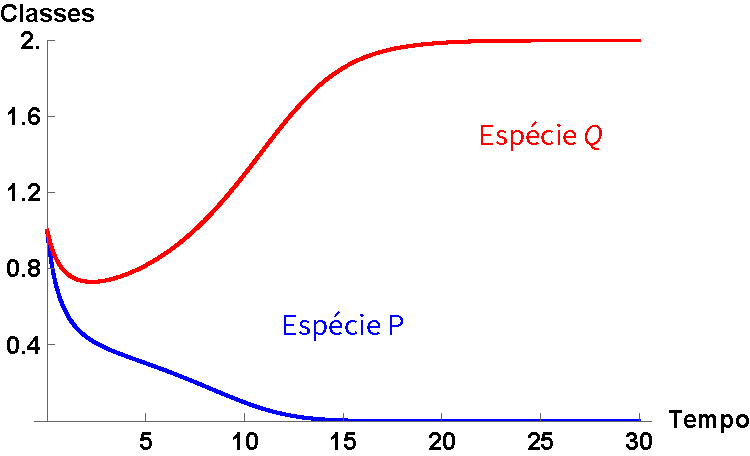
\includegraphics[keepaspectratio=true,scale=0.75]{caso1_a.pdf}
\caption{Solução numérica do sistema diferencial para o caso 1.}
\label{fig:x}
\end{figure}
\bigskip
\noindent
Comentario, Comentario,Comentario, Comentario,Comentario, Comentario,Comentario, Comentario,Comentario, Comentario,Comentario, Comentario,Comentario, Comentario,Comentario, Comentario,Comentario, Comentario,Comentario, Comentario,

%%%%%
\begin{figure}[htbp]
\centering
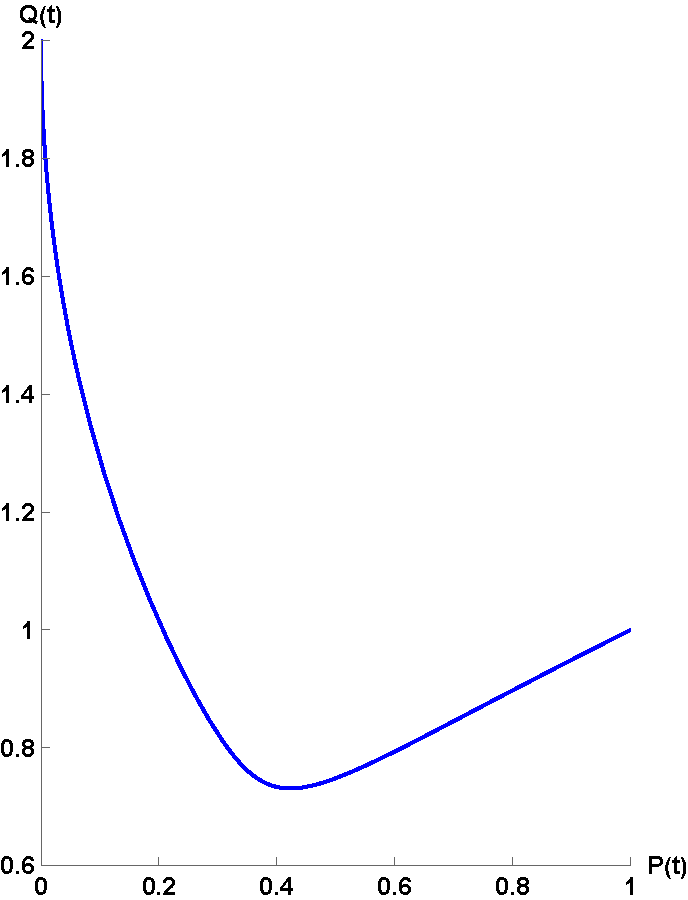
\includegraphics[keepaspectratio=true,scale=0.5]{caso1_b.pdf}
\caption{Esboço da relação entre P(t) e Q(t) para o caso 1.}
\label{fig:xx}
\end{figure}
\bigskip
\noindent
Comentario, Comentario,Comentario, Comentario,Comentario, Comentario,Comentario, Comentario,Comentario, Comentario,Comentario, Comentario,Comentario, Comentario,Comentario, Comentario,Comentario, Comentario,Comentario, Comentario,
\pagebreak


\begin{table}[h!]

\vspace*{0.25cm}

\begin{center}
\begin{tabular}{| c | c | c | c | c |}
\hline \hline
{Pontos de equilíbrio} & \multicolumn{2}{| c |}{Valores próprios} & {Tipo} & {Estabilidade}\\ \hline \hline

{$(0,0)$}   &   {$\lambda_1=0.5$} &   {$\lambda_2=1$}   &  {} & {Instável}\\ \hline

{$(0,2)$}   &   {$\lambda_1=-0.5$} &   {$\lambda_2=-1$}   &  {} & {Estável}\\ \hline

{$(1,0)$}   &   {$\lambda_1=-0.25$} &   {$\lambda_2=-1$}   &  {} & {Estável}\\ \hline

{$(0.5,0.5)$}   &   {$\lambda_1\cong-0.78$} &   {$\lambda_2\cong0.16$}   &  {Ponto de Sela} & {Instável}\\ \hline \hline

%%%%%
\end{tabular}
\end{center}
\label{tab:template}
\caption{Valores próprios e estabilidade por cada ponto de equilíbrio para o caso 1.}
\end{table}

\bigskip


\begin{figure}[htbp]
\centering
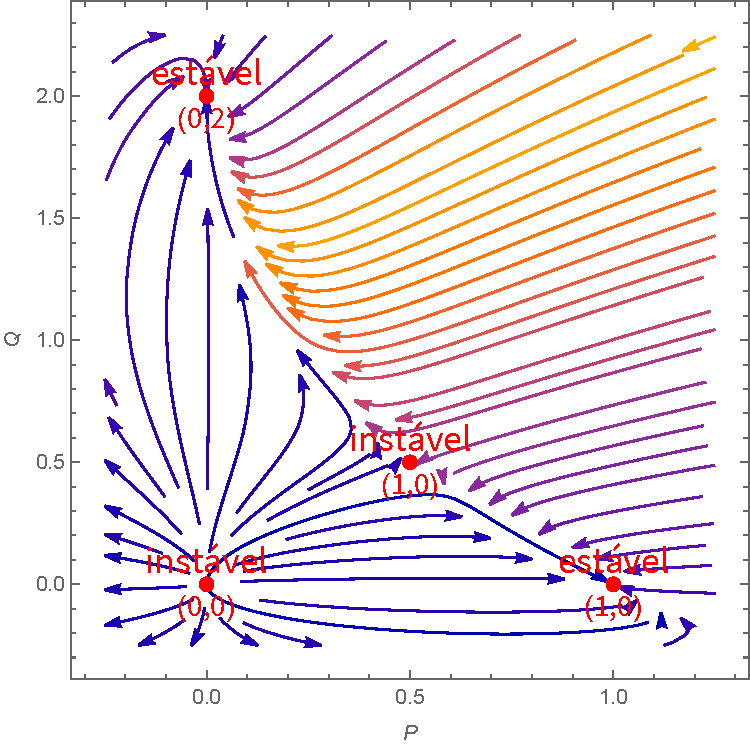
\includegraphics[keepaspectratio=true,scale=0.8]{caso1_c.pdf}
\caption{Campo de direções (com pontos de equilíbrio) para o caso 1.}
\label{fig:xxx}
\end{figure}
\bigskip
\noindent
Comentario, Comentario,Comentario, Comentario,Comentario, Comentario,Comentario, Comentario,Comentario, Comentario,Comentario, Comentario,Comentario, Comentario,Comentario, Comentario,Comentario, Comentario,Comentario, Comentario,
\pagebreak




















\subsubsection{Caso 2}


As condições iniciais são: $P(0)=Q(0)=1$.\newline Os parâmetros são:  $a=b=k=1$, $c=0.75$, $d=1$, $\ell=0.5$.
%%%%%
\begin{figure}[htbp]
\centering
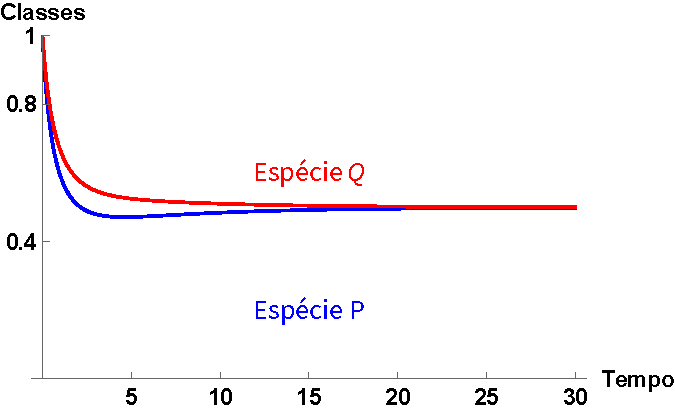
\includegraphics[keepaspectratio=true,scale=0.75]{caso2_a.pdf}
\caption{Solução numérica do sistema diferencial para o caso 2.}
\label{figy}
\end{figure}
\bigskip

\noindent
Comentario, Comentario,Comentario, Comentario,Comentario, Comentario,Comentario, Comentario,Comentario, Comentario,Comentario, Comentario,Comentario, Comentario,Comentario, Comentario,Comentario, Comentario,Comentario, Comentario,
%%%%%
\begin{figure}[htbp]
\centering
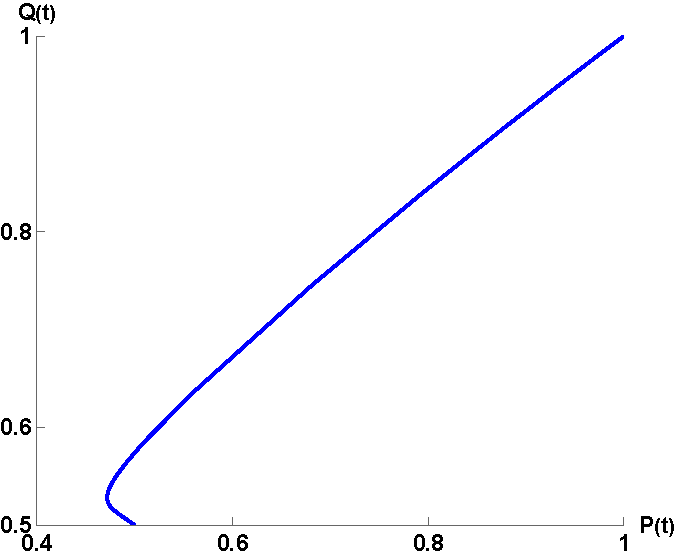
\includegraphics[keepaspectratio=true,scale=0.5]{caso2_b.pdf}
\caption{Esboço da relação entre P(t) e Q(t) para o caso 2.}
\label{fig:yy}
\end{figure}
\bigskip
\noindent
Comentario, Comentario,Comentario, Comentario,Comentario, Comentario,Comentario, Comentario,Comentario, Comentario,Comentario, Comentario,Comentario, Comentario,Comentario, Comentario,Comentario, Comentario,Comentario, Comentario,
\pagebreak
\begin{table}[h!]

\vspace*{0.25cm}

\begin{center}
\begin{tabular}{| c | c | c | c | c |}
\hline \hline
{Pontos de equilíbrio} & \multicolumn{2}{| c |}{Valores próprios} & {Tipo} & {Estabilidade}\\ \hline \hline

{$(0,0)$}   &   {$\lambda_1=0.75$} &   {$\lambda_2=1$}   &  {} & {Instável}\\ \hline

{$(0,0.75)$}   &   {$\lambda_1=-0.75$} &   {$\lambda_2=0.25$}   &  {Ponto de sela} & {Instável}\\ \hline

{$(1,0)$}   &   {$\lambda_1=-1$} &   {$\lambda_2=0.25$}   &  {Ponto de sela} & {Instável}\\ \hline

{$(0.5,0.5)$}   &   {$\lambda_1\cong-0.15$} &   {$\lambda_2\cong-0.86$}   &  {Ponto de Sela} & {Estável}\\ \hline \hline

%%%%%
\end{tabular}
\end{center}
\label{tab:template}
\caption{Valores próprios e estabilidade por cada ponto de equilíbrio para o caso 2.}
\end{table}

\bigskip
\begin{figure}[htbp]
\centering
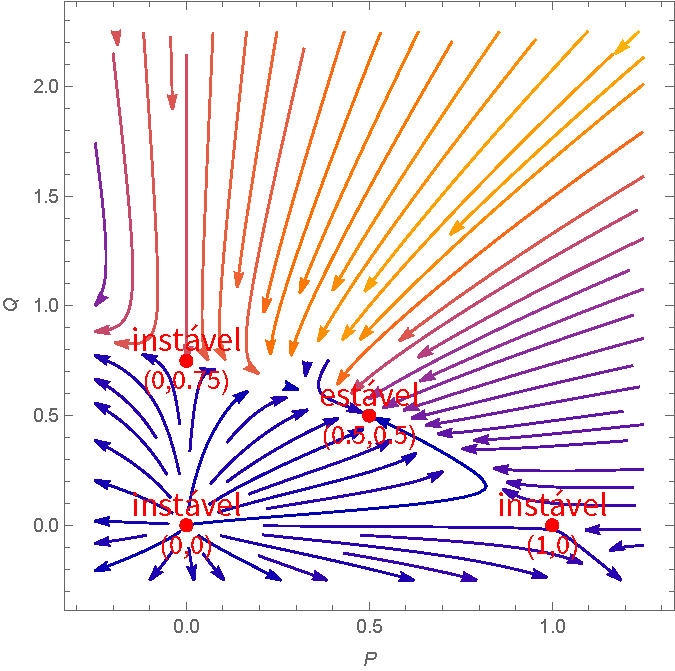
\includegraphics[keepaspectratio=true,scale=0.8]{caso2_c.pdf}
\caption{Campo de direções (com pontos de equilíbrio) para o caso 2.}
\label{fig:yyy}
\end{figure}
\bigskip
\noindent
Comentario, Comentario,Comentario, Comentario,Comentario, Comentario,Comentario, Comentario,Comentario, Comentario,Comentario, Comentario,Comentario, Comentario,Comentario, Comentario,Comentario, Comentario,Comentario, Comentario,




















\pagebreak
\subsubsection{Caso 3}


As condições iniciais são: $P(0)=Q(0)=1$.\newline Os parâmetros são:  $a=b=k=1$, $c=1.5$, $d=1$, $\ell=1$.
%%%%%
\begin{figure}[htbp]
\centering
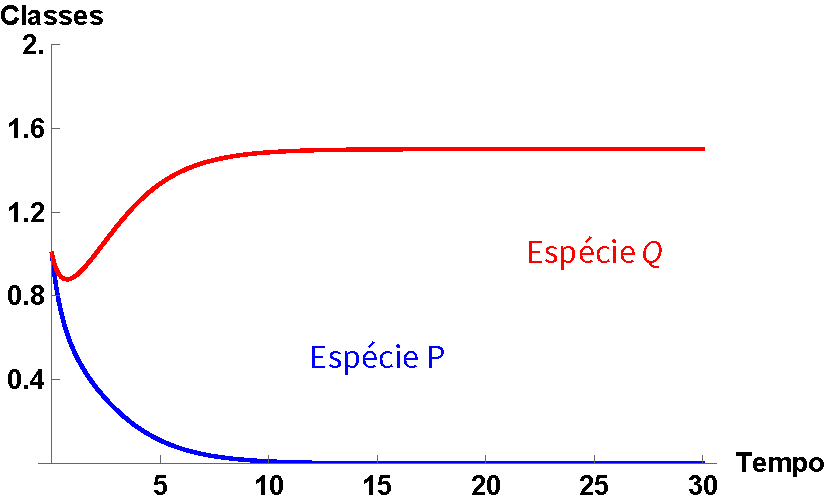
\includegraphics[keepaspectratio=true,scale=0.75]{caso3_a.pdf}
\caption{Solução numérica do sistema diferencial para o caso 3.}
\label{fig:z}
\end{figure}
\bigskip
\noindent
Comentario, Comentario,Comentario, Comentario,Comentario, Comentario,Comentario, Comentario,Comentario, Comentario,Comentario, Comentario,Comentario, Comentario,Comentario, Comentario,Comentario, Comentario,Comentario, Comentario,
\begin{figure}[htbp]
\centering
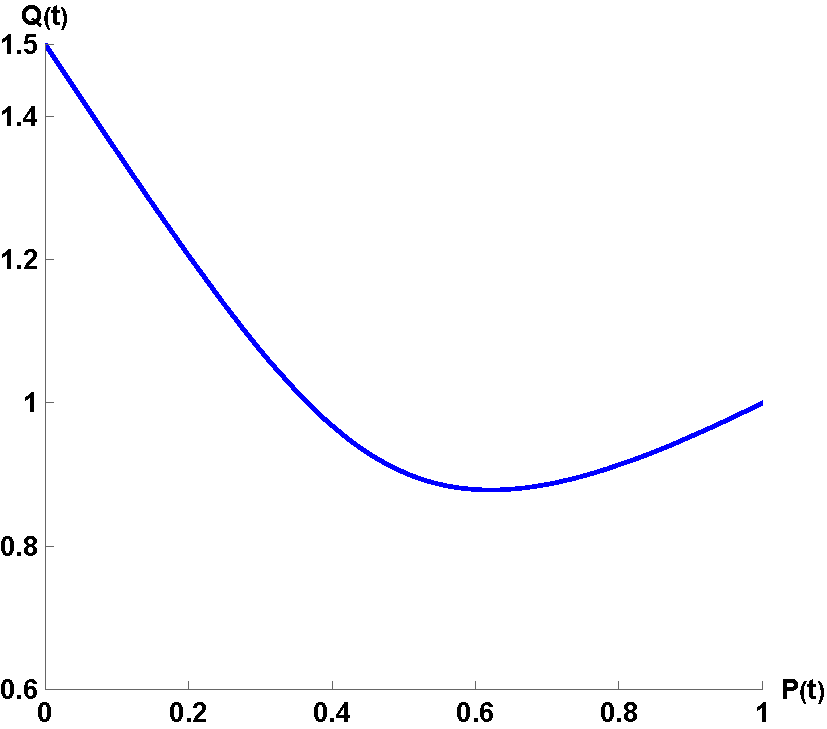
\includegraphics[keepaspectratio=true,scale=0.5]{caso3_b.pdf}
\caption{Esboço da relação entre P(t) e Q(t) para o caso 2.}
\label{fig:zz}
\end{figure}
\bigskip
\noindent
Comentario, Comentario,Comentario, Comentario,Comentario, Comentario,Comentario, Comentario,Comentario, Comentario,Comentario, Comentario,Comentario, Comentario,Comentario, Comentario,Comentario, Comentario,Comentario, Comentario,
\pagebreak
\begin{table}[h!]

\vspace*{0.25cm}

\begin{center}
\begin{tabular}{| c | c | c | c | c |}
\hline \hline
{Pontos de equilíbrio} & \multicolumn{2}{| c |}{Valores próprios} & {Tipo} & {Estabilidade}\\ \hline \hline

{$(0,0)$}   &   {$\lambda_1=1$} &   {$\lambda_2=1.5$}   &  {} & {Instável}\\ \hline

{$(0,1.5)$}   &   {$\lambda_1=-1.5$} &   {$\lambda_2=-0.5$}   &  {} & {Estável}\\ \hline

{$(1,0)$}   &   {$\lambda_1=-1.5$} &   {$\lambda_2=0.5$}   &  {Ponto de Sela} & {Instável}\\ \hline

{}   &   {} &   {}   &  {} & {}\\ \hline \hline

%%%%%
\end{tabular}
\end{center}
\label{tab:template}
\caption{Valores próprios e estabilidade por cada ponto de equilíbrio para o caso 3.}
\end{table}

\bigskip
%%%%%
\begin{figure}[htbp]
\centering
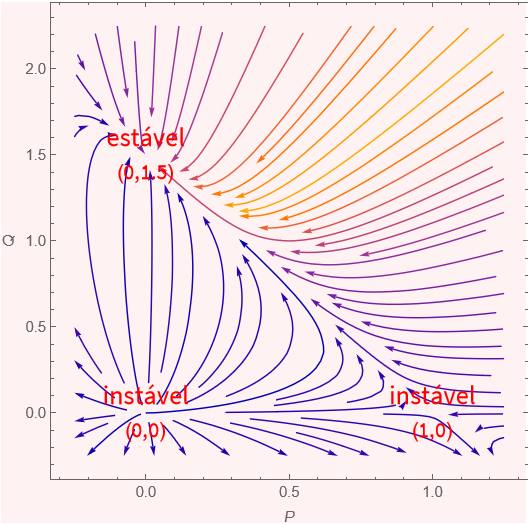
\includegraphics[keepaspectratio=true,scale=0.8]{caso3_c.jpg}
\caption{Campo de direções (com pontos de equilíbrio) para o caso 3.}
\label{fig:zzz}
\end{figure}
\bigskip
\noindent
Comentario, Comentario,Comentario, Comentario,Comentario, Comentario,Comentario, Comentario,Comentario, Comentario,Comentario, Comentario,Comentario, Comentario,Comentario, Comentario,Comentario, Comentario,Comentario, Comentario,

















\pagebreak
\subsubsection{Caso 4}


As condições iniciais são: $P(0)=Q(0)=2$.\newline Os parâmetros são:  $a=0.1$, $b=0.005$, $k=0.001$, $c=0.2$, $d=\frac{0.2}{120}$, $\ell=0.02$.
%%%%%
\begin{figure}[htbp]
\centering
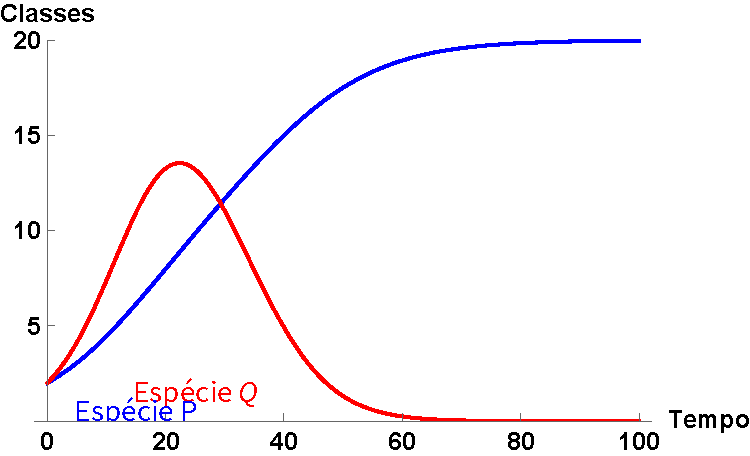
\includegraphics[keepaspectratio=true,scale=0.75]{caso4_a.pdf}
\caption{Solução numérica do sistema diferencial para o caso 4.}
\label{fig:w}
\end{figure}
\bigskip
\noindent
Comentario, Comentario,Comentario, Comentario,Comentario, Comentario,Comentario, Comentario,Comentario, Comentario,Comentario, Comentario,Comentario, Comentario,Comentario, Comentario,Comentario, Comentario,Comentario, Comentario,
%%%%%
\begin{figure}[htbp]
\centering
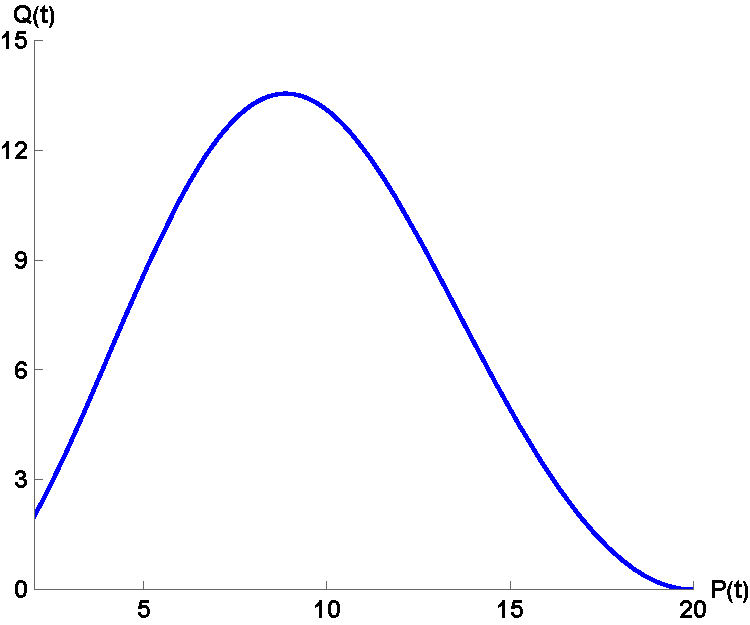
\includegraphics[keepaspectratio=true,scale=0.5]{caso4_b.pdf}
\caption{Esboço da relação entre P(t) e Q(t) para o caso 4.}
\label{fig:ww}
\end{figure}
\bigskip
\noindent
Comentario, Comentario,Comentario, Comentario,Comentario, Comentario,Comentario, Comentario,Comentario, Comentario,Comentario, Comentario,Comentario, Comentario,Comentario, Comentario,Comentario, Comentario,Comentario, Comentario,
\pagebreak
\begin{table}[h!]

\vspace*{0.25cm}

\begin{center}
\begin{tabular}{| c | c | c | c | c |}
\hline \hline
{Pontos de equilíbrio} & \multicolumn{2}{| c |}{Valores próprios} & {Tipo} & {Estabilidade}\\ \hline \hline

{$(0,0)$}   &   {$\lambda_1=0.1$} &   {$\lambda_2=0.2$}   &  {} & {Instável}\\ \hline

{$(0,120)$}   &   {$\lambda_1=-0.2$} &   {$\lambda_2=-0.02$}   &  {} & {Estável}\\ \hline

{$(20,0)$}   &   {$\lambda_1=-0.1$} &   {$\lambda_2=-0.2$}   &  {} & {Estável}\\ \hline

{$(2.86,85.7)$}   &   {$\lambda_1\cong-0.02$} &   {$\lambda_2\cong-0.17$}   &  {Ponto de Sela} & {Instável}\\ \hline \hline

%%%%%
\end{tabular}
\end{center}
\label{tab:template}
\caption{Valores próprios e estabilidade por cada ponto de equilíbrio para o caso 4.}
\end{table}

%%%%%
\begin{figure}[htbp]
\centering
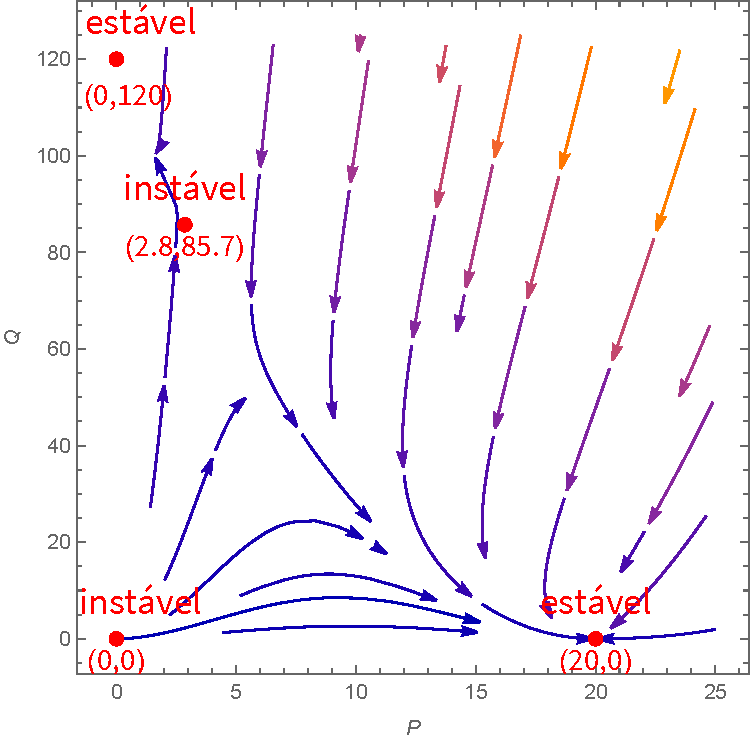
\includegraphics[keepaspectratio=true,scale=0.8]{caso4_c.pdf}
\caption{Campo de direções (com pontos de equilíbrio) para o caso 4.}
\label{fig:www}
\end{figure}
\bigskip
\noindent
Comentario, Comentario,Comentario, Comentario,Comentario, Comentario,Comentario, Comentario,Comentario, Comentario,Comentario, Comentario,Comentario, Comentario,Comentario, Comentario,Comentario, Comentario,Comentario, Comentario,


\pagebreak

\section{Conclusão}
\pagebreak

%\bigskip

%\noindent
%Para a Bibliografia, \'e conveniente usar automatismos, como se faz a seguir.

%\noindent
%Devo incluir Livros como em \cite{livro}, Artigos como em \cite{artigo}, Notas como em \cite{nota} \& Apontamentos.
%Se tiver Teses, fa\c co como em \cite{tese} 
%Outros textos de apoio.
%Informa\c c\~ao dispon\'\i vel em {\it sites} de Internet, como em \cite{site}.
%Etc.

%\bigskip

%\noindent
%{\color{ggreen}Depois da Bibliografia, inclu\'\i \ f\'ormulas matem\'aticas e outras coisas \'uteis.}

%%%%%%%%%%%%%%

\begin{thebibliography}{99}

%\bibitem{livro} 
%A. Autor e B. Autor,
%{\it T\'\i tulo do livro}, Wiley, New York, 2012.

%\bibitem{artigo} 
%A. Autor e B. Autor,
%``T\'\i tulo do artigo na revista'', {\it Nome da Revista},  Vol.~000, No.~00 (2012), pp. 0000-0000.

%\bibitem{nota} 
%A. Autor, B. Autor e C. Autor,
%``T\'\i tulo da Nota'', {\it T\'\i tulo da confer\^encia}, 
%AMS Proceedings, Vol.~000, 2012, Eds. A.A.~Editor1, B.B.~Editor2, pp. 00-00.

%\bibitem{tese} 
%A. Autor,
%``T\'\i tulo da tese'', Tese de Mestrado ou de Doutoramento, Universidade, Pa\'\i s, 2012.

%\bibitem{site} 
%Informa\c c\~ao que \`a data tal e tal estava dispon\'\i vel no seguinte site de categoria
%\url{https://www.google.pt/}  

%\bibitem{site-SANDRO} 
%Titulo. [Online].
%\url{https://www.google.pt/}  

\bibitem{wolfram} 
Wolfram One. [Online].
\url{https://www.wolfram.com/wolfram-one/}  

\bibitem{latex} 
Project Latex. [Online].
\url{https://www.latex-project.org/about/}  

\bibitem{overleaf} 
Overleaf. [Online].
\url{https://www.overleaf.com/about/}  

\bibitem{matlab} 
Matlab. [Online].
\url{https://www.mathworks.com/discovery/what-is-matlab.html/}  

%https://www.overleaf.com/about

%https://www.wolfram.com/wolfram-one/
%https://www.latex-project.org/about/

%Boyce & DePrima, Elementary Differential Equations and Boundary Value Problems
\bibitem{boyce} 
Boyce \& DePrima,
{\it Elementary Differential Equations and Boundary Value Problems}


\bibitem{livro22} 
Ana Jacinta Soares,
{\it Cálculo (A e B), MIEEIC, MIECOM, 2007/2008 : notas sobre a disciplina}, Departamento de Matemática, Universidade do Minho, 2007.

\bibitem{livro2}
Gaspar J. Machado,
{\it Tópicos de Álgebra Linear e Geometria Analítica}, Departamento de Matemática e Aplicações, Universidade do Minho, 2014.
%\bibitem{artigo2} 
%``Statistical Journal'', {\it REVSTAT},  Vol.~17, No.~2 (2019), pp. 145-162.


\bibitem{livro2} 
Jorgue Figueiredo e Carolina Ribeiro,
{\it Apontamentos de Equações Diferenciais (Complementos de Análise Matemática EE)}, Departamento de Matemática e Aplicações, Universidade do Minho, 2013.

\bibitem{livro2} 
N. Baca\"{e}r,
{\it A Short History of Mathematical Population Dynamics}, DOI 10.1007/978-0-85729-115-8 6, © Springer-Verlag London Limited, 2011.

\bibitem{livro2} 
Robert Zwanzig,
{\it Generalized Verhulst Laws for Population Growth (competition)}, Institute for Fluid Dynamics and Applied Mathematics, University of Maryland, College Park Md. 20742, 1973.

%\bibitem{livro2} 
%Robert Zwanzig,
%{\it Generalized Verhulst Laws for Population Growth (competition)}, Institute for Fluid Dynamics and Applied Mathematics, University of Maryland, College Park Md. 20742, 1973.





%\bibitem{sitee} 
%Khan Academy,
%\url{https://www.khanacademy.org/science/ap-biology/ecology-ap/population-ecology-ap/a/exponential-logistic-growth} 



%https://www.khanacademy.org/science/ap-biology/ecology-ap/population-ecology-ap/a/exponential-logistic-growth


%\bibitem{livroaaaa} 
%Ana Jacinta Soares,
%{\it Cálculo (A e B), MIEEIC, MIECOM, 2007/2008 : notas sobre a disciplina}, Departamento de Matemática, Universidade do Minho, 2007.


\end{thebibliography}

\pagebreak


%%%%%
%\input{project_plan}


%CONDICOES INICIAIS

%\begin{table}[h!]

%\vspace*{0.25cm}

%\begin{center}
%\begin{tabular}{| c | c | c | c | c |}
%\hline \hline
%{\small Caso}  &  {\small 1}   &   {\small 2}   &  {\small 3}   &  {\small 4} 
%\\ \hline \hline
%$P(0)$  &  $1$ & $1$  & $1$  & $2$
%\\ \hline
%$Q(0)$  &  $1$ & $1$  & $1$  & $2$
%\\ \hline
%$a$  &  $1$ & $1$  & $1$  & $0,1$
%\\ \hline
%$b$  &  $1$ & $1$  & $1$  & $0,05$
%\\ \hline
%$c$  &  $0,5$ & $0,75$  & $1,5$  & $0,2$ 
%\\ \hline
%$d$  &  $0,25$ & $1$  & $1$  & $0,2/120$
%\\ \hline
%$k$  &  $1$ & $1$  & $1$  & $0,001$
%\\ \hline
%$\ell$  &  $0,75$ & $0,5$  & $1$  & $0,02$
%\\ \hline \hline 
%%%%%
%\end{tabular}
%\end{center}
%\label{tab1}
%\caption{Aqui escrevo a legenda desta tabela.}
%\end{table}
%\bigskip


%\section{Conclusão}




\end{document}








